\documentclass[12pt,prb,aps,epsf]{article}
\usepackage[utf8]{inputenc}
\usepackage{amsmath}
\usepackage{amsfonts}
\usepackage{amssymb}
\usepackage{graphicx} 
\usepackage{latexsym} 
\usepackage[toc,page]{appendix}
\usepackage{listings}
\usepackage{xcolor}
\usepackage{soul}
\usepackage[T1]{fontenc}
\usepackage{amsthm}
\usepackage{mathtools}
\usepackage{setspace}
\usepackage{array,multirow,makecell}
\usepackage{geometry}
\usepackage{textcomp}
\usepackage{float}
%\usepackage{siunitx}
\usepackage{cancel}
%\usepackage{tikz}
%\usetikzlibrary{calc, shapes, backgrounds, arrows, decorations.pathmorphing, positioning, fit, petri, tikzmark}
\usepackage{here}
\usepackage{titlesec}
%\usepackage{bm}
\usepackage{bbold}

\geometry{hmargin=2cm,vmargin=2cm}

\begin{document}
	
	\title{LP 32 Microscopies optiques}
	\author{Mathevet}
	
	\maketitle
	
	\tableofcontents
	
	\pagebreak
	

\subsection{Introduction}
Situer le contexte, on va étudier un instrument d'optique.\\
Instrument d'optique : palier les limitations de l'oeil, microscope : voir de petits objets.\\
16e s premiers microscope, en fait de grosses loupes, ou une goutte de miel ou de résine : lentille sphérique. Il faut attendre le milieu du 19e s pour voir apparaître des microscopes composés, constitués d'un objectif qui collecte la lumière de l'objet et forme une image intermédiaire, et d'un oculaire qui joue le rôle de loupe pour observer l'image intermédiaire.\\

Motivation : grossir beaucoup = voir des grands angles, tout en limitant les aberrations. Les microscopes sont donc des instruments complexes formés de différents objets : lentilles, diaphragmes, doublets ect...

\section{Lois de l'optique géométriques appliquées à un modèle de microscope}
\begin{figure}
	\centerline{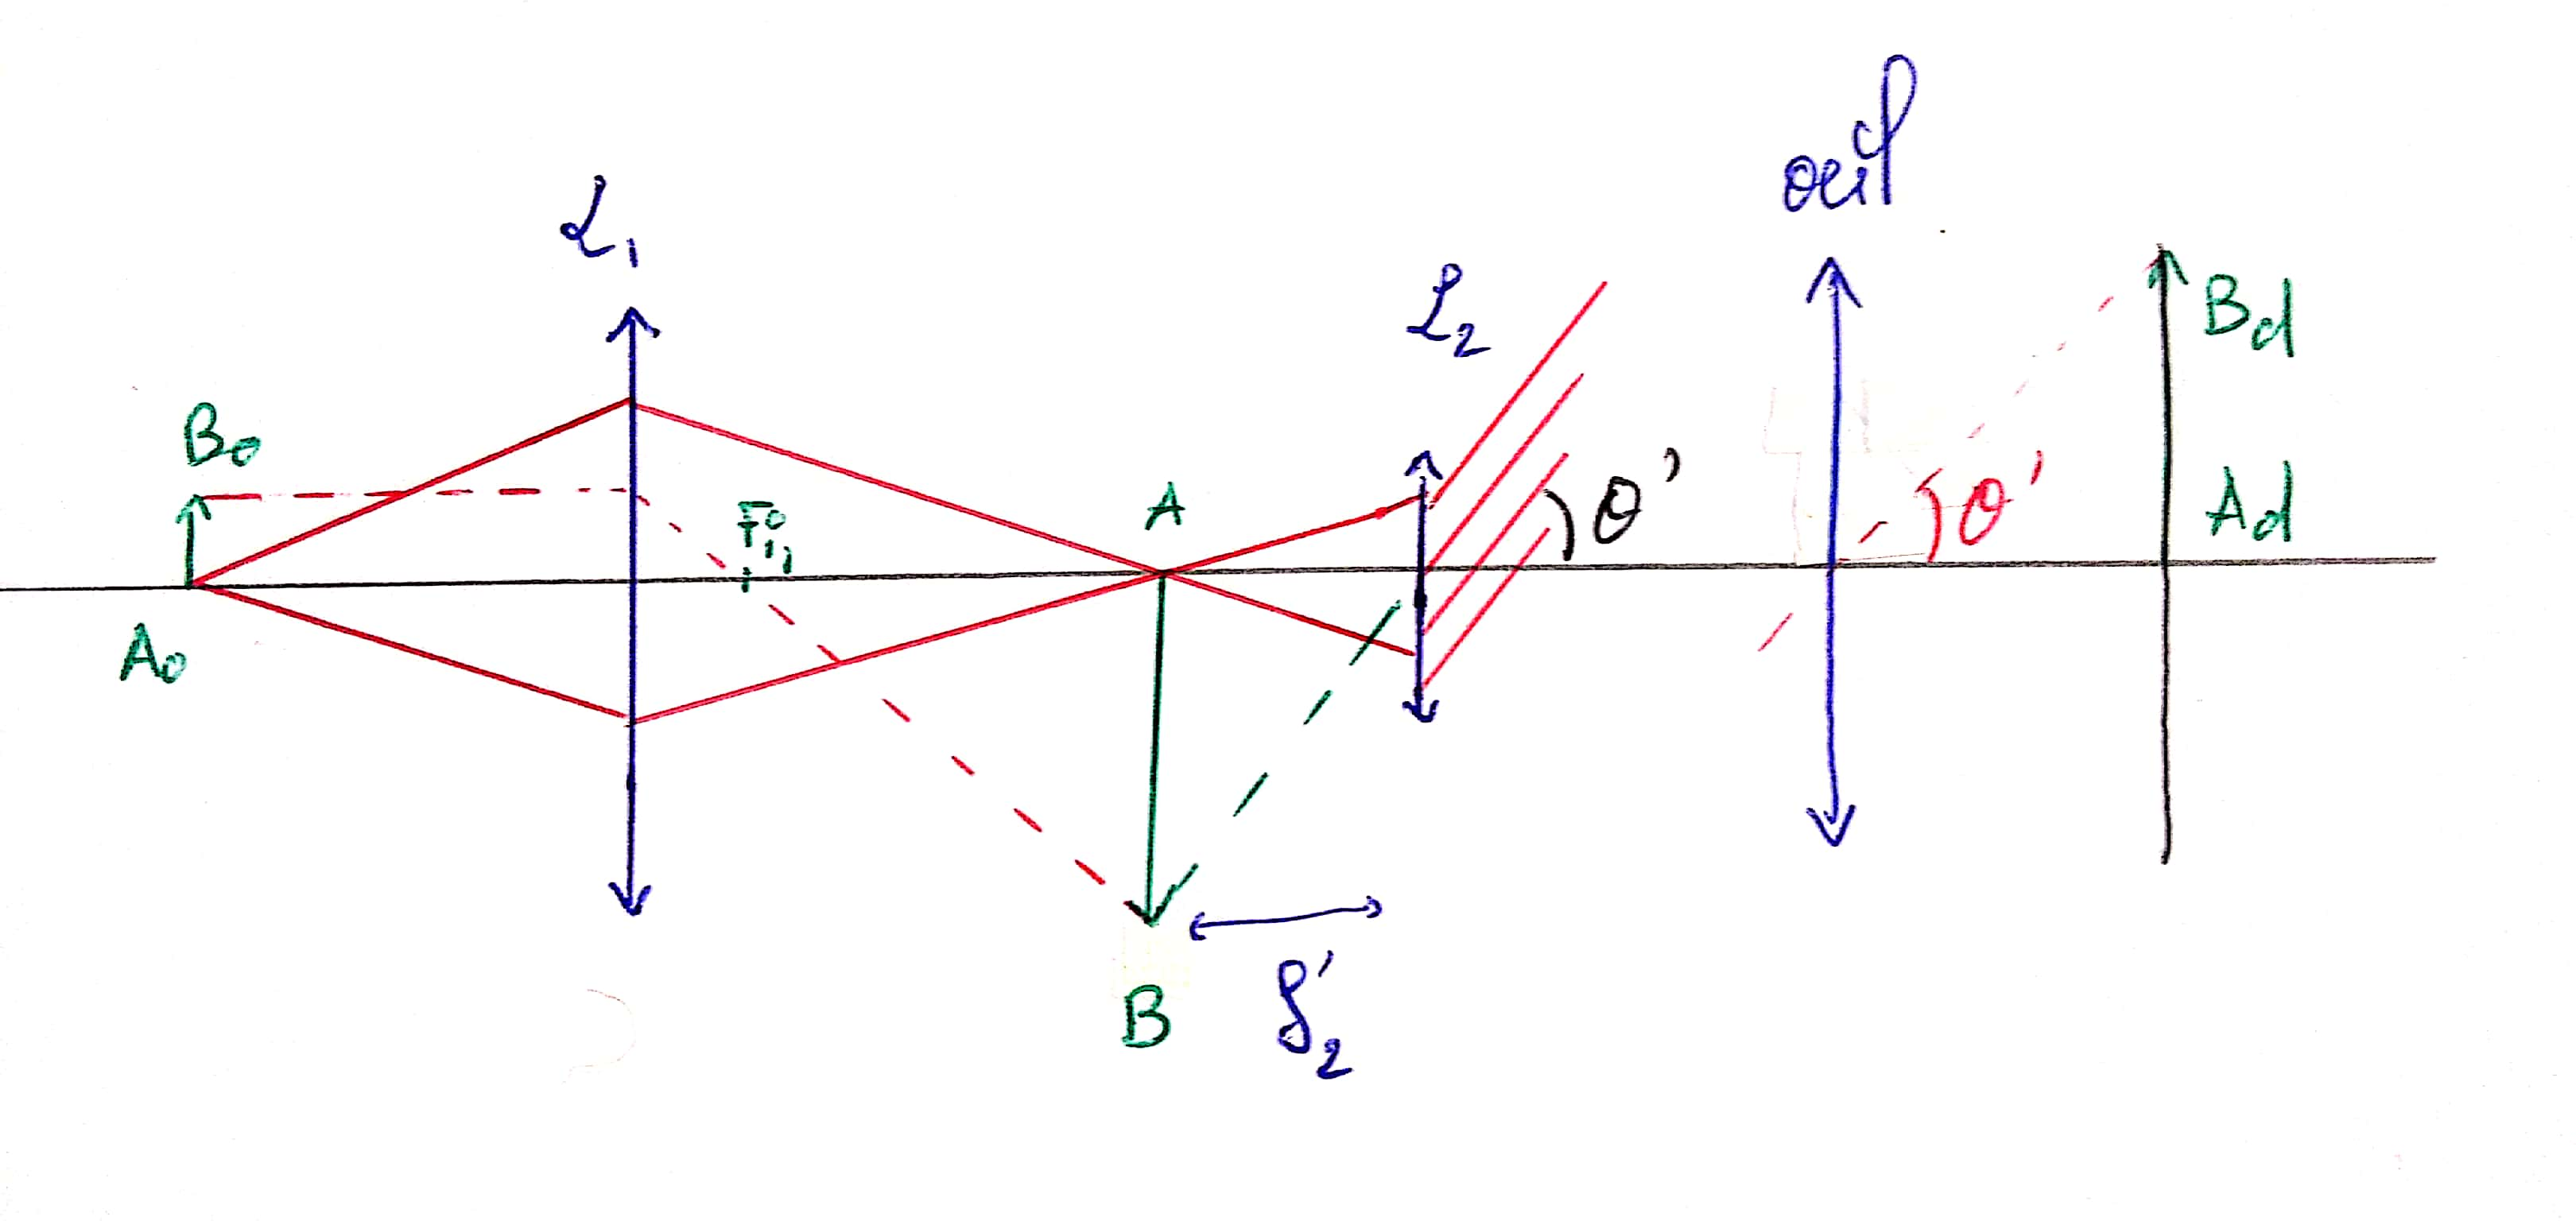
\includegraphics[width=15cm]{schema}}
\end{figure}
\subsection{Constitution}
schéma dans le Houard\\
Puissance d'un microscope : $P = \frac{\theta'}{A_0B_0} = \frac{\theta'}{AB}
\frac{AB}{A_0B_0} = P_{oc}G_{obj}$ avec $P_{oc}=1/f_{oc}$.

\subsection{Applications des lois}
On a $\gamma_{obj} = \frac{F_{i1}A}{f_{obj}} = -\frac{F_{i1}F_{o2}}{f_{obj}}$ (Newton)\\
$P_{microscope} = -\frac{\Delta}{f_{obj}f_{oc}}$ : on augmente la puissance en prenant de courtes focales, et on aura donc de grosses inclinaisons.\\

\subsection{Expérimentation du modèle}
\subsubsection{Modèle de l'œil}
On sait que l'oeil est au repos lorsqu'il regarde une image à l'infini. Il faut donc autocollimater, en formant l'image de A par L1, L2 et une réflection sur un miroir dans le plan contenant l'objet.\\
%On peut résumer le montage oeil plus microscope par $A\rightarrow \infty \rightarrow \infty \rightarrow A'$(dans l'oeil)
Au final on a, avec l'oeil 
\begin{eqnarray}
\gamma_d = \frac{A_dB_d}{A_0B_0} = \frac{f_{oeil}\Delta}{f_{oc}f_{obj}}
\end{eqnarray}

\subsubsection{Mesures}

\subsection{Objectif réel}
On a le problème des aberrations, il faut donc remplir 2 conditions : 

Stigmatisme rigoureux, réalisé, pour les lentilles boules pour les deux points de Weierstrass, pb : un des deux points est dans la lentille boule. Astuce : on scie la boule et on supprime le dioptre générée par la coupe en mettant la boule dans une huile ayant le même indice optique que le verre qui constitue la boule, et en mettant l'objet au niveau du point maintenant dans l'huile. (Voir figure 7.19 du Houard). On complète ensuite avec un ménisque d'amicii et un doublet de Lister, qui est un doublet achromatique collé, dans lequel on a 3 rayons de courbure, 2 indices et 2 constringences ($\nu = \frac{\Delta n}{n-1}$ : variation de l'indice avec la "profondeur"), on a deux contraintes : on veut que le doublet soit achromatique, on impose $f_i$, il reste 5 paramètres ajustables, dont on se sert pour les aberrations sphériques.

\subsubsection{Diaphragme d'ouverture}
C'est le diaphragme qui limite la quantité de lumière qui passe par le système.\\
Manip pour les montages : on met un diaphragme d'ouverture réglable, et on montre qu'en sortie du microscope on observe le même champs, mais pas avec la même luminosité, mesure au fluxmètre.

\subsection{Oculaires réels}
\subsubsection{Achromatisme}
Ce sont en général des doublets, de focales $f_1$ et $f_2$ et séparés par la distance $e$. On a une condition d'achromatisme : voir après figure 7.29.

\subsubsection{Verre de champ}
A ce point on peut faire la manip du \textbf{verre de champ}. On met une lentille dans le plan ou se forme l'image par l'objectif, ce qui ne change pas la conjugaison, mais qui permet de rabattre les rayons, et ainsi le limiter l'effet de diaphragme de champ que va provoquer $L_2$.

\subsubsection{Cercle oculaire}
L'idée est ici de répondre à la question : "où placer son œil ?"\\
Cercle oculaire = pupille de sortie : zone le plus petite par laquelle tous les rayons passent en sortie du microscope, c'est l'image du diaphragme d'ouverture.

\section{Limite de résolution}
\subsection{Diffraction}
On pourrait se dire, qu'avec beaucoup de moyens on pourrait avoir un grandissement infini... mais non, dans la pratique on sera limité par la diffraction.

Voir démo Pérez pour la limite de diffraction.

\subsection{Mise en évidence expérimentale}
Pour les montages : \textbf{Manip d'Abbes = filtrage spatial}\\

Jusqu'au années 2000 il était accepté que la limitations ultime serait la limite de diffraction.

\subsection{Battre la limite de diffraction}
\subsubsection{PALM}
Voir diapo "CD".

\subsubsection{STED}
Pour PALM et STED aller voir sur wikipedia, et Vincent Croquet.

On va ici chercher à localiser plus qu'à voir les molécules : on a changé de paradigme.

\section{Conclusion}
Ouvrir sur le fait que l'on peut maintenant sonder la matière avec d'autres particules que le photons.

\subsection{Différentes méthodes}
On peut aussi regarder le spectre de chaque "point", sa polarisation, sa phase (voir contrainte de phase dans le cours de Mathevet), on peut aussi regarder ver d'autres phénomènes non linéaires.
\section{Références}
\begin{itemize}
	\item Optique de sylvain Houard
	\item Optique de Pérez
\end{itemize}

\section{Remarques}
Il faut adapter en quarante minutes, on ne peut donc faire qu'une manip.

	
\end{document}